\subsubsection{Detection \& Segmentation.}
ED enables integrating sensors through the use of the plugins present in the ed\_sensor\_integration package. Two different plugins exist:
1. The \emph{laser\_plugin}: Enables tracking of 2D laser clusters. This plugin can be used to track dynamic obstacles such as humans.
2. The \emph{kinect\_plugin}: Enables world model updates with use of data from the Microsoft Kinect\texttrademark. This plugin exposes several ROS services that realize different functionalities:
\begin{enumerate}[label=(\alph*)]
\item Segment: A service that segments sensor data that is not associated with other world model entities. Segmentation areas can be specified per entity in the scene. This allows to segment object ‘on-top-of’ or ‘in’ a cabinet.
\item FitModel: A service that fits the specified model in the sensor data of the Microsoft Kinect\texttrademark. This allows updating semi-static obstacles such as tables and chairs.
\end{enumerate}


The \emph{ed\_sensor\_integration} plugins enable updating and creating entities. However, new entities are classified as unknown entities.
%\begin{figure}[h]
%    \centering
%    %\vspace{-0.3cm}
%	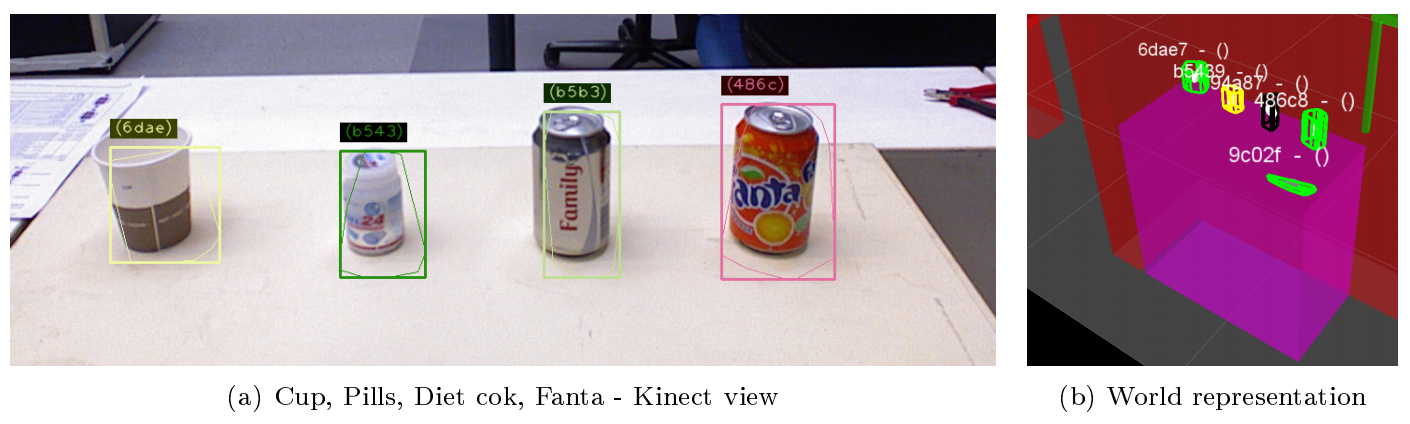
\includegraphics[width = 1\linewidth]{Figures/ed_perception}
%    %\vspace{-1em}
%    \caption{ED Perception responsible for the object segmentation and calling the object recognition service. Left, the segmented objects in the robot's sensor frame are displayed; the final annotated world representation is shown in the right picture.}
%	\label{fig:ed_perception}
%    %\vspace{-0.5cm}
%\end{figure} 